\section{Consenso Promedio en Sistemas Holonómicos}
\onecolumn
\subsection{Grafo completamente conexo}
Protocolo de consenso de vecino más cercano de Jadbabaie et al.~\cite{jadbabaie2003}, con agentes integradores en el plano:
\begin{align*}
    \dot{\mathbf{x}}_i &= \mathbf{u}_i \\[6pt]
    \mathbf{u}_i &=
    \underbrace{\sum_{j \in \mathcal{N}_i} a_{ij}\,(\mathbf{x}_j-\mathbf{x}_i)}_{\text{\footnotesize Atracción a los vecinos}}
\end{align*}

Cuando los cuatro agentes se perciben entre sí, el grafo es conexo y el protocolo converge al promedio real de las posiciones iniciales, de acuerdo con las condiciones de convergencia de matrices estocásticas de Wolfowitz~\cite{wolfowitz1963}.

\begin{figure}[H]
    \centering
    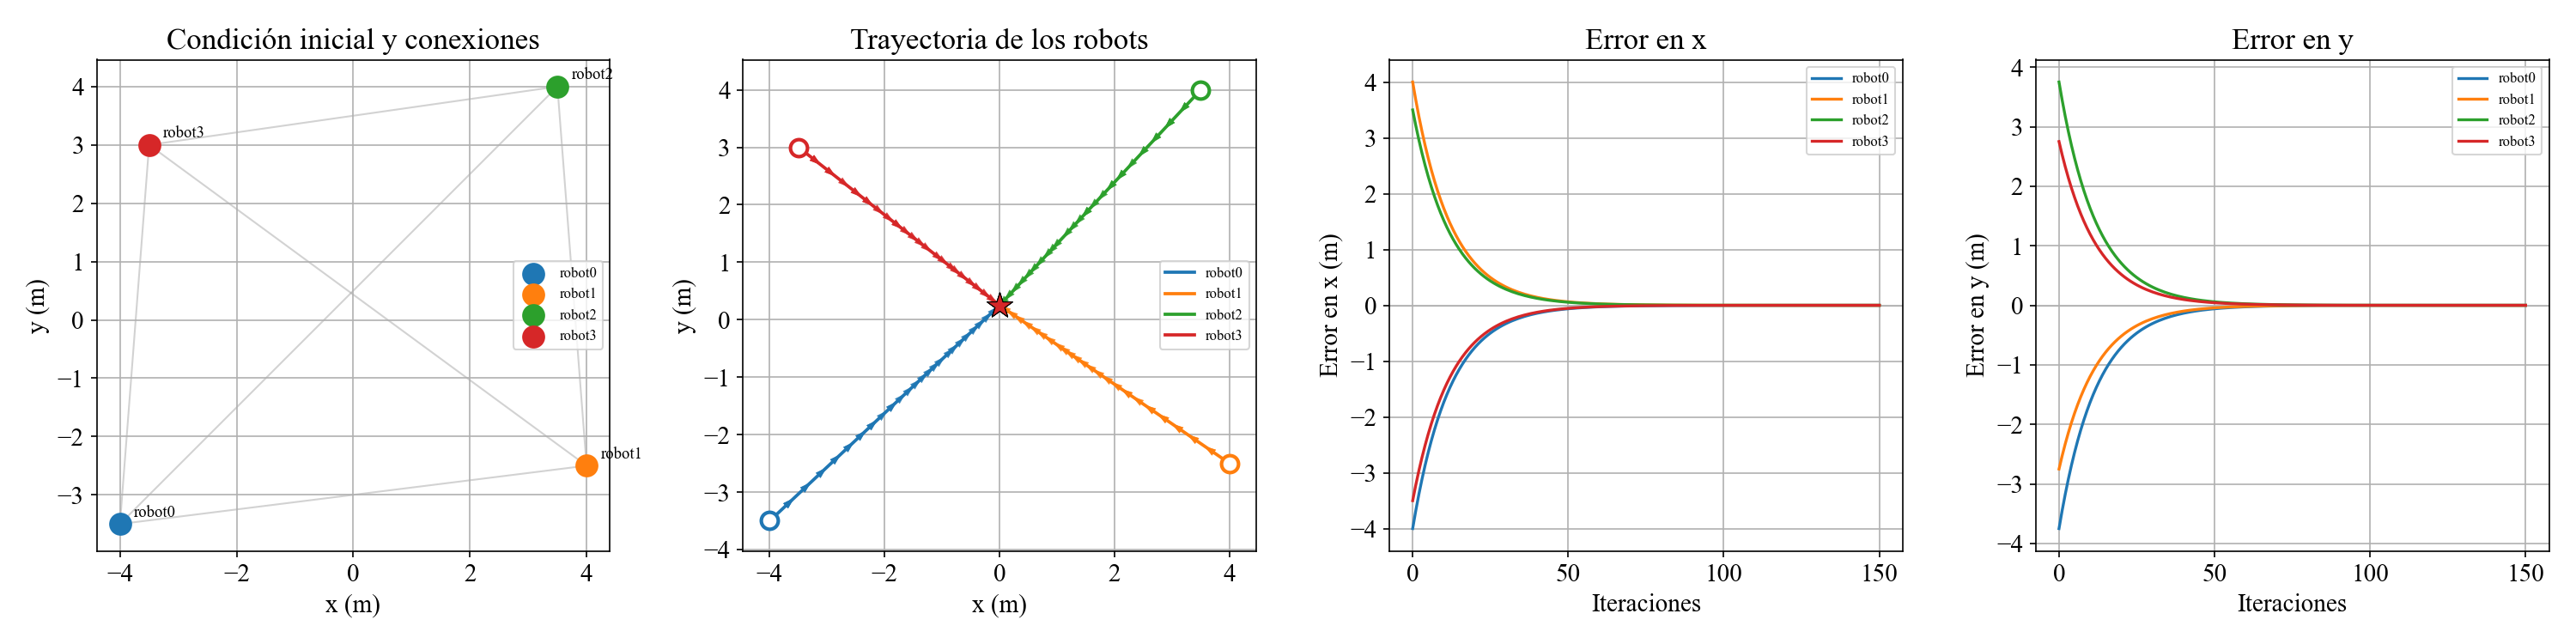
\includegraphics[width=\linewidth]{Pics/consenso_promedio_fully (1).png}
    \caption{Con grafo completamente conexo, los cuatro agentes convergen al promedio real de sus posiciones iniciales.}
    \label{fig:consenso_fully}
\end{figure}

\section{Consenso Promedio en Sistemas Holonómicos}
\onecolumn
\subsection{Grafo parcialmente conexo}
Mismo protocolo y mismas condiciones iniciales, pero con un grafo en estrella donde solo el agente central percibe al resto.

\begin{figure}[H]
    \centering
    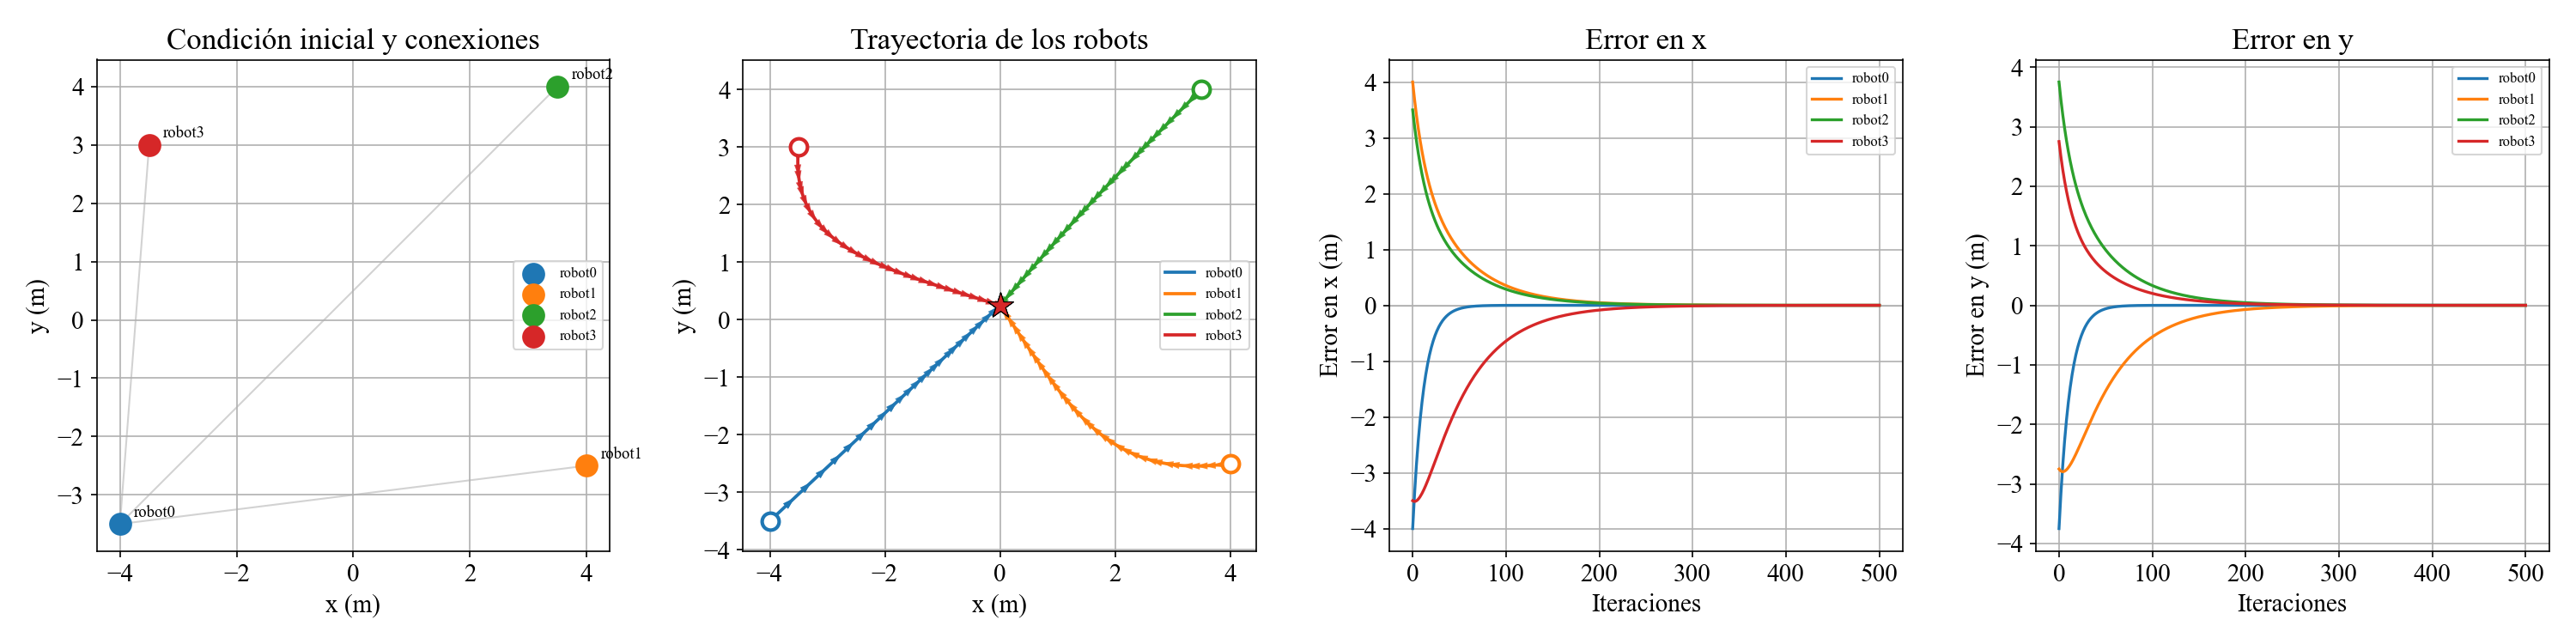
\includegraphics[width=0.75\linewidth]{Pics/consenso_promedio_mid (1).png}
    \caption{Con un grafo más disperso se llega al mismo promedio, pero en más iteraciones por la menor conectividad algebraica.}
    \label{fig:consenso_mid}
\end{figure}

\section{Consenso Promedio en Sistemas Holonómicos}
\onecolumn
\subsection{Agente aislado}
Se anula la percepción de un agente. Deja de escuchar a los demás y nunca se mueve, aunque el resto sí lo escucha:
\begin{align*}
    \dot{\mathbf{x}}_i &= \mathbf{u}_i \\[6pt]
    \mathbf{u}_i &=
    \underbrace{\sum_{j \in \mathcal{N}_i} a_{ij}\,(\mathbf{x}_j-\mathbf{x}_i)}_{\text{\footnotesize Atracción a los vecinos}}
    ,\qquad \mathbf{u}_1 = 0
\end{align*}

El agente aislado actúa como ancla fija. El grupo ya no converge al promedio real de los cuatro, sino hacia la posición de ese agente. La conectividad del grafo determina el valor de consenso.

\begin{figure}[H]
    \centering
    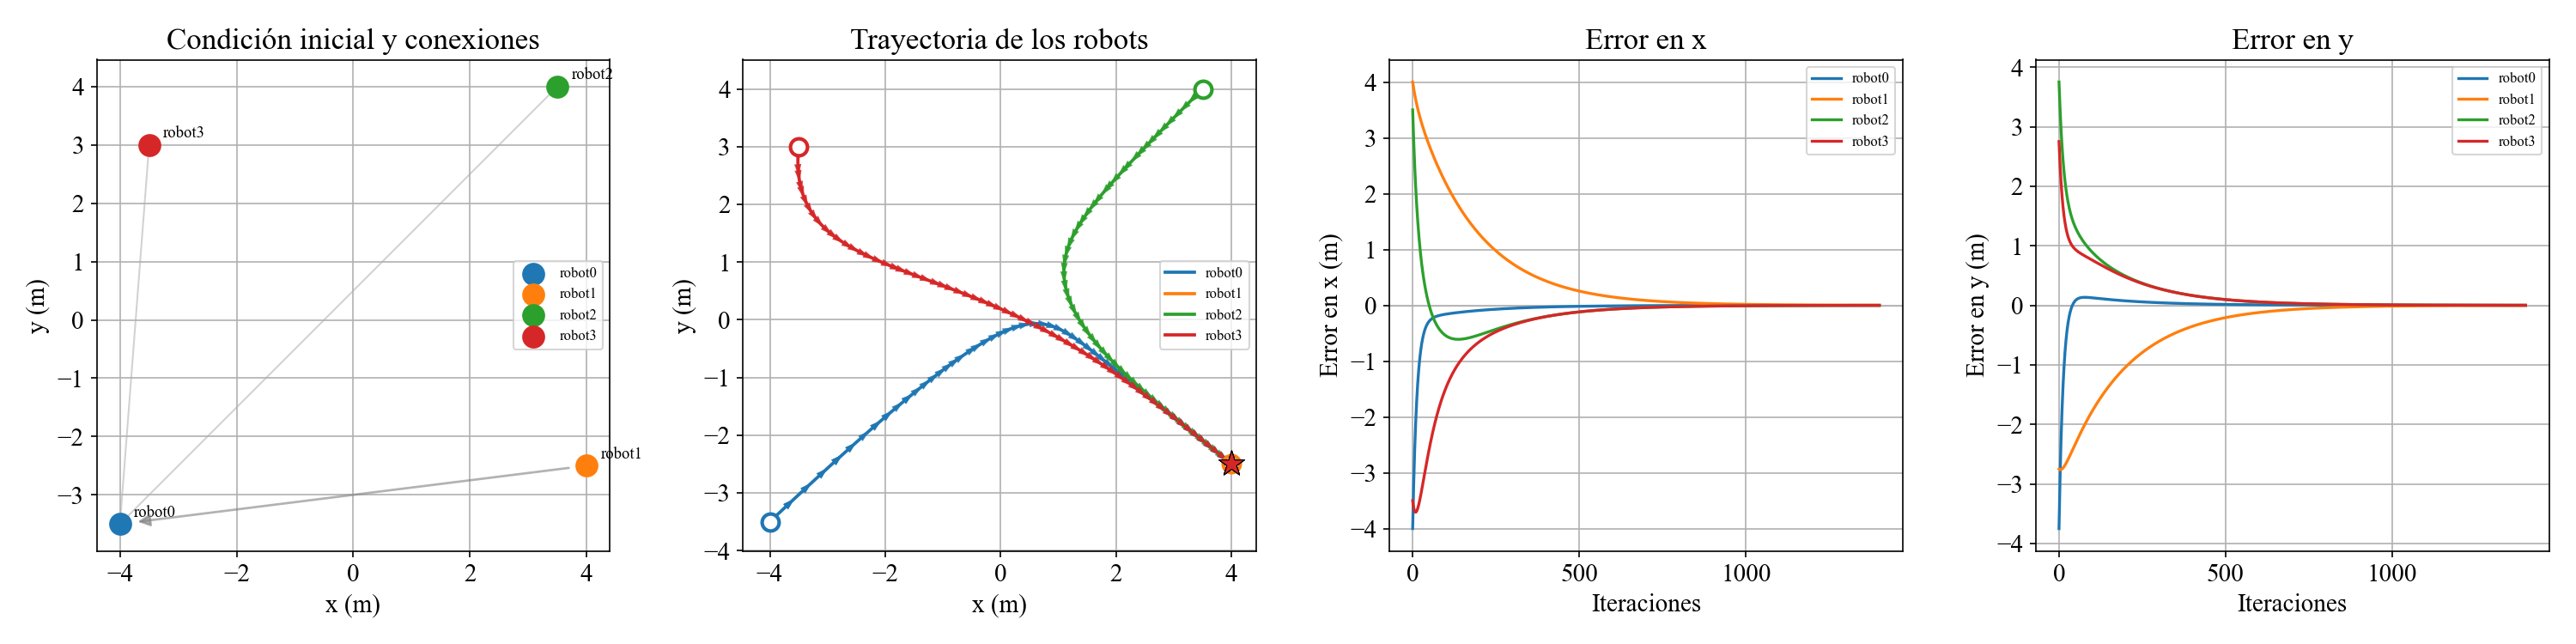
\includegraphics[width=\linewidth]{Pics/consenso_promedio_not (1).png}
    \caption{Al aislar un agente, el resto converge hacia su posición fija en vez del promedio real del grupo.}
    \label{fig:consenso_aislado}
\end{figure}

\section{Consenso con Seguimiento de Líder}
\onecolumn
\subsection{Líder con metas secuenciales}
Se introduce un líder que recorre una ruta de metas. Los seguidores hacen consenso entre sí y son atraídos hacia la posición actual del líder, no hacia la meta:
\begin{align*}
    \dot{\mathbf{x}}_i &= \mathbf{u}_i \\[6pt]
    \mathbf{u}_i &=
    \underbrace{\sum_{j \in \mathcal{N}_i} a_{ij}\,(\mathbf{x}_j-\mathbf{x}_i)}_{\text{\footnotesize Consenso entre seguidores}}
    \;\;
    \underbrace{+\,\beta\, b_i^0\,(\mathbf{x}_0-\mathbf{x}_i)}_{\text{\footnotesize Atracción al líder}}
\end{align*}

El líder $\mathbf{x}_0$ avanza hacia cada meta con control proporcional. Los seguidores lo persiguen manteniendo el consenso entre sí. La atracción al líder desplaza el valor de consenso del grupo hacia una referencia móvil.

\begin{figure}[H]
    \centering
    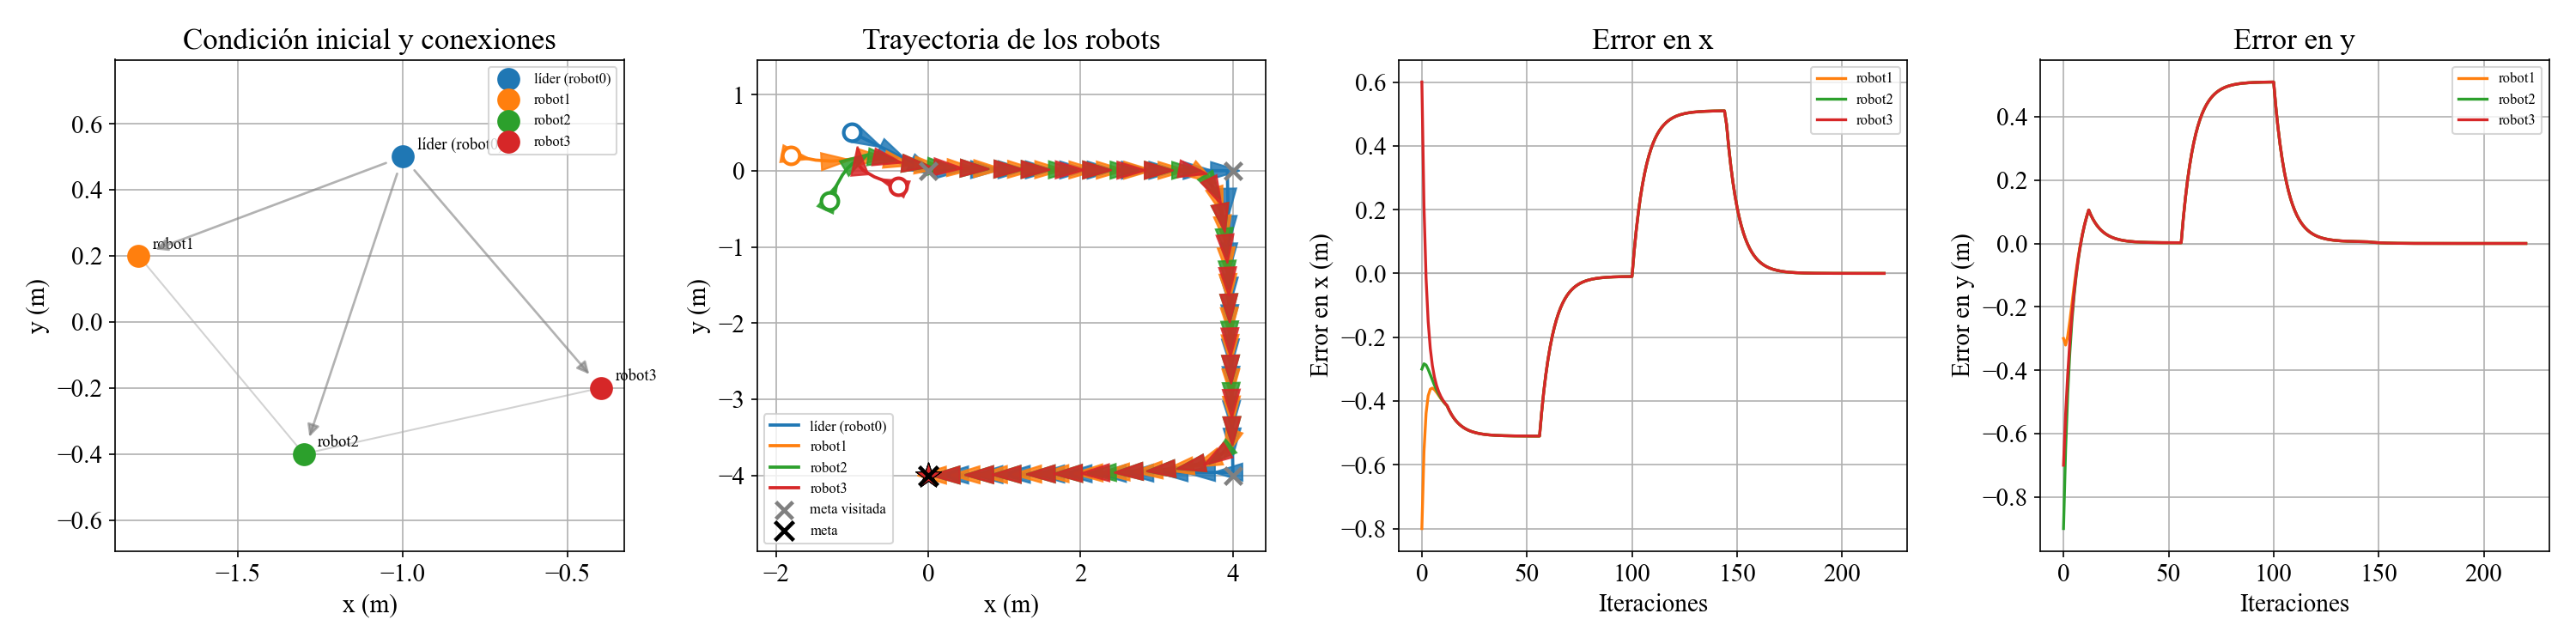
\includegraphics[width=\linewidth]{Pics/lider_seguidor_multimeta_mid3 (1).png}
    \caption{El líder recorre cuatro metas secuenciales mientras los seguidores lo persiguen manteniendo el consenso entre sí.}
    \label{fig:lider_seguidor}
\end{figure}

\section{Control de Formaciones con Consenso en Sistemas Holonómicos}
\onecolumn
\subsection{Consenso con mantenimiento de formación}
Se parte del protocolo de Armel et al.~\cite{koulong2024distributed} y se modifica para agentes integradores, con $\nu_1=1$ y $\nu_2=\beta$:
\begin{align*}
    \dot{\mathbf{x}}_i &= \mathbf{u}_i \\[6pt]
    \mathbf{u}_i &=
    \underbrace{-\sum_{j \in \mathcal{N}_i} a_{ij}\big[(\mathbf{x}_i-\mathbf{r}_i)-(\mathbf{x}_j-\mathbf{r}_j)\big]}_{\text{\footnotesize Consenso entre vecinos}}
    \;\;
    \underbrace{-\,\beta\, b_i^0\big[(\mathbf{x}_i-\mathbf{r}_i)-\mathbf{x}_0\big]}_{\text{\footnotesize Atracción al ancla virtual}}
\end{align*}

Como antes, el desplazamiento $\mathbf{r}_i$ evita que el consenso colapse a los agentes en un punto y los sitúa en su lugar dentro de la formación. La diferencia: el ancla $\mathbf{x}_0$ es ahora virtual y común, y solo la perciben los agentes con $b_i^0=1$.

\begin{figure}[H]
    \centering
    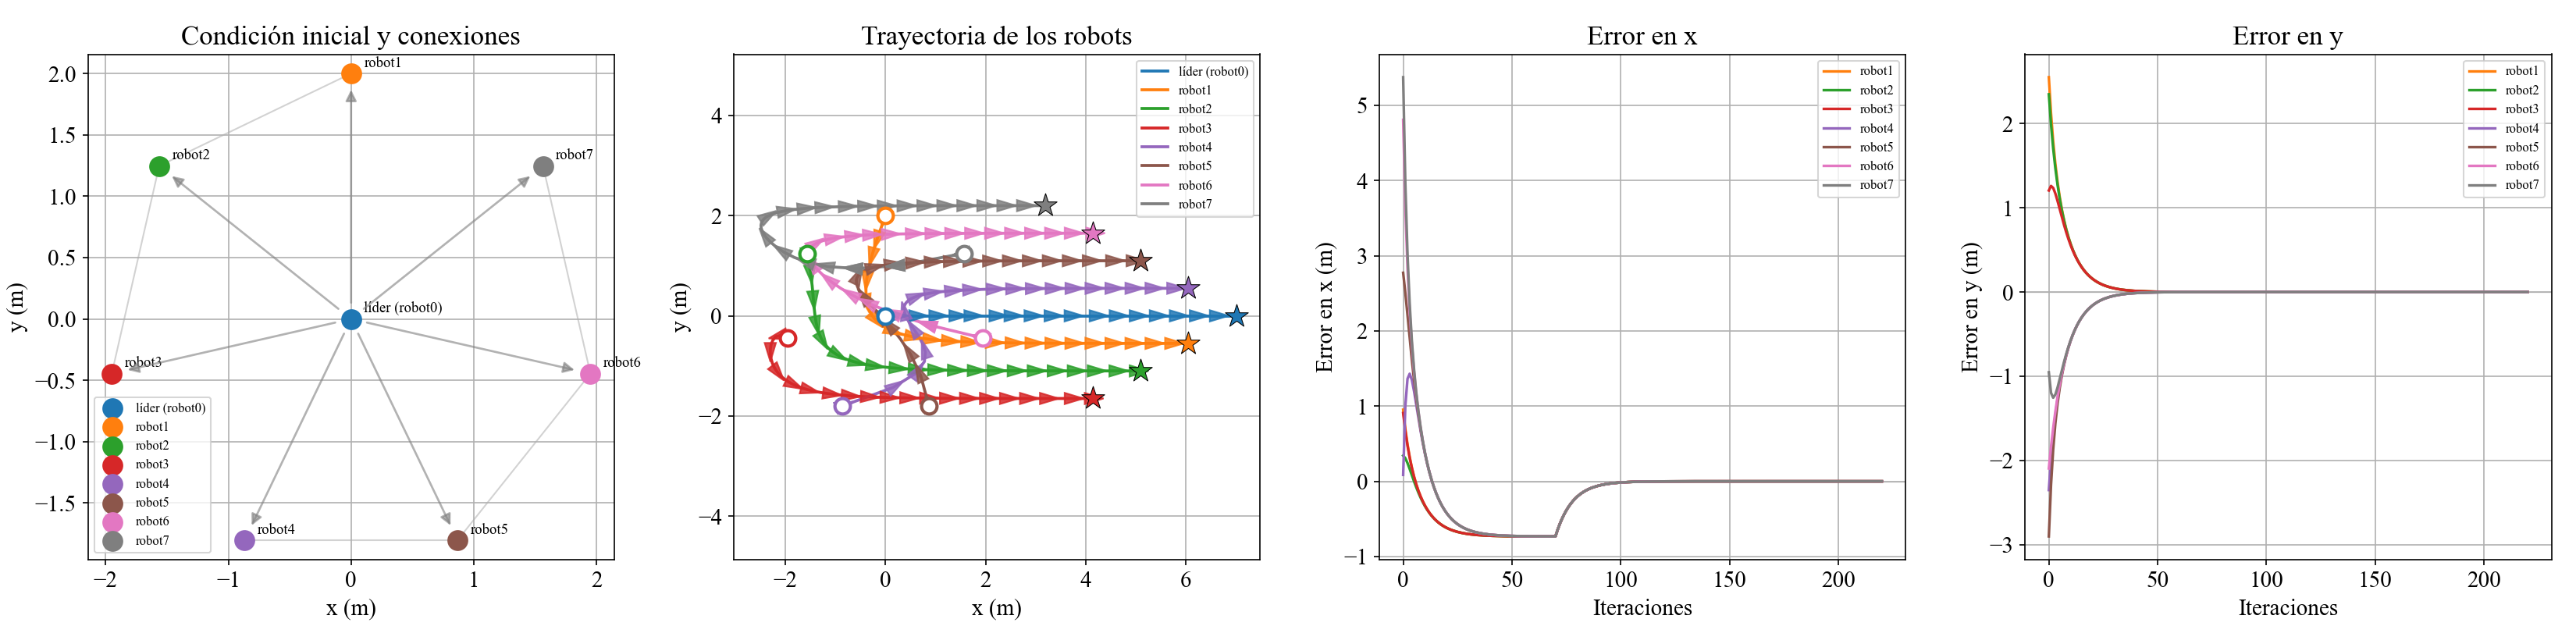
\includegraphics[width=\linewidth]{Pics/anclas_virtuales_resultado.png}
    \caption{Seguidores convergen hacia sus anclas virtuales}
    \label{fig:anclas_virtuales}
\end{figure}

\section{Control de Formaciones con Consenso en Sistemas Holonómicos}
\onecolumn
\subsection{Consenso con mantenimiento de formación}
Significado de cada símbolo de la ley de control:
\begin{align*}
    \dot{\mathbf{x}}_i &= \mathbf{u}_i \\[6pt]
    \mathbf{u}_i &=
    \underbrace{-\sum_{j \in \mathcal{N}_i} a_{ij}\big[(\mathbf{x}_i-\mathbf{r}_i)-(\mathbf{x}_j-\mathbf{r}_j)\big]}_{\text{\footnotesize Consenso entre vecinos}}
    \;\;
    \underbrace{-\,\beta\, b_i^0\big[(\mathbf{x}_i-\mathbf{r}_i)-\mathbf{x}_0\big]}_{\text{\footnotesize Atracción al ancla virtual}}
\end{align*}

{\footnotesize
\noindent
\begin{tabular}{l@{\ }l@{\qquad}l@{\ }l}
$\mathbf{x}_i,\mathbf{x}_j$ & posición de $i$ y $j$ & $\mathcal{N}_i$ & vecinos del agente $i$ \\
$\dot{\mathbf{x}}_i=\mathbf{u}_i$ & velocidad de control & $a_{ij}$ & peso de comunicación $i$--$j$ \\
$\mathbf{r}_i,\mathbf{r}_j$ & desplazamiento en la formación & $b_i^0$ & $1$ si $i$ percibe el ancla \\
$\mathbf{x}_0$ & ancla virtual común & $\beta$ & ganancia de atracción al ancla \\
\end{tabular}
}

\section{Control de Formaciones con Consenso en Sistemas No Holonómicos}
\onecolumn
\subsection{Efecto Látigo y Noción de Líder Físico}
Error de formación sobre errores relativos, con atracción a un líder físico:
\begin{equation*}
    \mathbf{e}_i = -\sum_{j \in \mathcal{N}_i} a_{ij}\big[(\mathbf{x}_i - \mathbf{r}_i) - (\mathbf{x}_j - \mathbf{r}_j)\big] - \beta\,b_i^0\big[(\mathbf{x}_i - \mathbf{r}_i) - \mathbf{x}_0\big]\end{equation*}

Como cada seguidor persigue una posición referida al líder, un giro brusco de este se propaga en cadena y se amplifica hacia los extremos de la formación: el efecto látigo.
\begin{figure*}[h]
    \centering
    
\includegraphics[width=0.9\textwidth]{/home/calafaker/Control-Formation/documentacion/figuras/personales/formacion_latigo.pdf}
    \caption{Simulación de protocolo de consenso de errores relativos}
    \label{fig:consensus_results}
\end{figure*}